%
% Capítulo 3a - Metodologías y Tecnologías
%
\chapter[Metodologías y Tecnologías]{
	Metodologías y Tecnologías
	\label{cap:metodologia}
}

En el presente capítulo se va a justificar la metodología seguida en la definición e implementación del proyecto, así como las tecnologías software empleadas.

% ----------------------------------
% Sec Metodología
% ----------------------------------
\section{Metodologías} % (fold)
  \label{sec:metodologias}

  Para asegurar el éxito durante el desarrollo de software no es suficiente contar con notaciones de modelado y herramientas, hace falta un elemento importante: la {\bf metodología de desarrollo}, la cual nos provee de una dirección a seguir para la correcta aplicación de los demás elementos.

  	Generalmente el proceso de desarrollo llevaba asociado un marcado énfasis en el control del proceso mediante una rigurosa definición de roles, actividades y artefactos, incluyendo modelado y documentación detallada. Este esquema «tradicional» para abordar el desarrollo de software ha demostrado ser efectivo y necesario en proyectos de gran tamaño (respecto a tiempo y recursos), donde por lo general se exige un alto grado de ceremonia en el proceso. Sin embargo, este enfoque no resulta ser el más adecuado para muchos de los proyectos actuales donde el entorno del sistema es muy cambiante, y en donde se exige reducir drásticamente los tiempos de desarrollo pero manteniendo una alta calidad.

  	Ante las dificultades para utilizar metodologías tradicionales con estas restricciones de tiempo y flexibilidad, muchos equipos de desarrollo se resignan a prescindir de las buenas prácticas de la Ingeniería del Software, asumiendo el riesgo que ello	conlleva. 

  A la hora de afrontar el desarrollo de este Proyecto Fin de Carrera, se han evaluado las dos metodologías más usadas actualmente para elegir la que más se ajusta al desarrollo.
  
  % ----------------------------------
  % Sub Proceso Unificado de Desarrollo
  % ----------------------------------
  \subsection{Proceso Unificado de Desarrollo} % (fold)
    \label{sub:proceso_unificado_de_desarrollo}
    
    El Proceso Unificado de Desarrollo de Software (PUD) es una metodología para acometer el desarrollo de sistemas informáticos, propuesta por Ivar Jacobson, Grady Booch y James Rumbaugh. Tiene las siguientes características:
    
    \begin{itemize}
      \item Se trata de un estándar avalado por la OMG, {\it Object Management Group}, consorcio de alrededor de 800 miembros (compañías de la industria del software), que busca el desarrollo de especificaciones para la industria del software que sea técnicamente excelentes, comercialmente viables e independientes del vendedor. OMG define {\it object management} como el desarrollo software que modela el mundo real mediante su representación como objetos. Estos objetos no son más que el encapsulamiento de atributos, relaciones y métodos de componentes software identificables.
      \item Recoge la experiencia de tres grandes metodologías anteriores: {\it OMG (Object Modeling Technique)} de Rumbaugh, {\it OOAD (Object-Oriented Analysis and Design)} de Booch y {\it Objectory} de Jacobson.
       \item Actualmente se usa en la mayoría de las empresas para grandes proyectos y se imparte por muchas instituciones.
    \end{itemize}
  
    El PUD es un {\bf proceso de desarrollo software}. Un proceso de desarrollo de software es el conjunto de actividades necesarias para transformar los requisitos de un usuario en un sistema software. Sin embargo, el proceso unificado es más que un proceso de trabajo, es un marco de trabajo genérico que puede especializarse para una gran variedad de sistemas software, para diferentes áreas de aplicación, diferentes tipos de organizaciones y diferentes niveles de aptitud.
  
    El PUD está basado en componentes y utiliza UML. Está dirigido por casos de uso, porque con éstos se especifican las funcionalidades que el sistema proporciona al usuario. Los casos de uso representan los requisitos funcionales y fuerzan a pensar en términos de importancia para el usuario y no sólo en términos de funciones que sería bueno tener. Los casos de uso no sólo son una herramienta para especificar los requisitos del sistema, sino que también guían su diseño, implementación y prueba. En conclusión se podría decir que guían el desarrollo software.
  
    El PUD está centrado en la arquitectura, pues la manera en que se organiza el sistema depende de los casos de uso clave y debe en tener en cuenta la comprensibilidad, la facilidad de adaptación al cambio y la reutilización. Los casos de uso clave son aquellos que dotan al sistema con la funcionalidad fundamental para los usuarios y sin los cuales, los demás casos de uso no tienen sentido.
  
    El PUD es iterativo e incremental. El trabajo se divide en partes más pequeñas llamadas iteraciones. En cada iteración se recorren los flujos de trabajo (requisitos, análisis y diseño, implementación y pruebas) y se obtiene una versión interna. En síntesis, en cada iteración se amplía el sistema con nuevos casos de uso, se identifican nuevos riesgos y se mitigan los ya conocidos. Las iteraciones se agrupan en fases, que por orden secuencial son las siguientes: {\it inicio, elaboración, construcción y transición}. Cada una centra sus esfuerzos más en unos flujos de trabajo que en otros. La etapa de inicio se centra en la captura de requisitos y él análisis. La etapa de elaboración lo hace con el análisis y el diseño. Las etapas de construcción y transición se centran en el diseño, implementación y pruebas.
  
    El PUD es una metodología de desarrollo pensada para proyectos grandes, a largo plazo  y con un equipo de desarrollo numeroso.

  % subsection proceso_unificado_de_desarrollo (end)

  % ----------------------------------
  % Sub Metodologías Ágiles
  % ----------------------------------
  \subsection{Metodologías Ágiles} % (fold)
    \label{sub:metodologias_agiles}
    
    A principios de la década del ’90, surgió un enfoque que fue bastante revolucionario para su momento ya que iba en contra de toda creencia de que mediante procesos altamente definidos se iba a lograr obtener software en tiempo, costo y con la requerida calidad. El enfoque fue planteado por primera vez por J. Martin (Nueva York, 1991)  y se dio a conocer en la comunidad de Ingeniería de Software con el nombre de RAD o {\it Rapid Application Development}. RAD consistía en un entorno de desarrollo altamente productivo, en el que participaban grupos pequeños de programadores utilizando herramientas que generaban código en forma automática tomando como entradas sintaxis de alto nivel. En general, se considera que este fue uno de los primeros hitos en pos de la agilidad en los procesos de desarrollo.
    
    La historia de las Metodologías Ágiles y su apreciación como tales en la comunidad de la Ingeniería de Software tiene sus inicios en la creación de una de las metodologías utilizada como arquetipo: {\it XP - eXtreme Programming}, que nace de la mente de Kent Beck, tomando ideas recopiladas junto a Ward Cunningham.

    Durante 1996, Beck es llamado por Chrysler como asesor del proyecto {\it Chrysler Comprehensive Compensation (C3) payroll system}. Dada la poca calidad del sistema que se estaba desarrollando, Beck decide tirar todo el código y empezar de cero utilizando las prácticas que él había ido definiendo a lo largo del tiempo. El sistema, que administra la liquidación de aproximadamente 10.000 empleados, y consiste de 2.000 clases y 30.000 métodos, es puesto en operación en Mayo de 1997 casi respetando el calendario propuesto. Como consecuencia del éxito de dicho proyecto, Kent Beck dio origen a XP iniciando el movimiento de metodologías ágiles al que se anexarían otras metodologías surgidas mucho antes que el propio Beck fuera convocado por Chrysler.
    	
    Es así como que este tipo de metodologías fueron inicialmente llamadas «metodologías livianas». Sin embargo, aun no contaban con una aprobación, pues se le consideraba por muchos desarrolladores como meramente intuitiva. Luego, con el pasar de los años, en febrero de 2001, tras una reunión celebrada en Utah-EEUU, nace formalmente el término «ágil» aplicado al desarrollo de software. En esta misma reunión participan un grupo de 17 expertos de la industria del software, incluyendo algunos de los creadores o impulsores de metodologías de software con el objetivo de esbozar los valores y principios que deberían permitir a los equipos desarrollar software rápidamente y respondiendo a los cambios que puedan surgir a lo largo del proyecto. Se pretendía ofrecer una alternativa a los procesos de desarrollo de software tradicionales, caracterizados por ser rígidos y dirigidos por la documentación que se genera en cada una de las actividades desarrolladas.

    Tras esta reunión se creó {\it The Agile Alliance}, una organización, sin ánimo de lucro, dedicada a promover los conceptos relacionados con el desarrollo ágil de software y ayudar a las organizaciones para que adopten dichos conceptos. El punto de partida fue el Manifiesto Ágil, un documento que resume la filosofía «ágil».
    
    % ----------------------------------
    % SubSub El Manifiesto Ágil
    % ----------------------------------
    \subsubsection{El Manifiesto Ágil} % (fold)
    \label{ssub:el_manifiesto_agil}
    
      Según el Manifiesto se valora:
      
      \begin{itemize}
        \item {\bf Al individuo y las interacciones del equipo de desarrollo sobre el proceso y las herramientas.} La gente es el principal factor de éxito de un proyecto software. Es más importante construir un buen equipo que construir el entorno. Muchas veces se comete el error de construir primero el entorno y esperar que el equipo se adapte automáticamente. Es mejor crear el equipo y que éste configure su propio entorno de desarrollo en base a sus necesidades.
        \item {\bf Desarrollar software que funciona más que conseguir una buena documentación}. La regla a seguir es «no producir documentos a menos que sean necesarios de forma inmediata para tomar un decisión importante». Estos documentos deben ser cortos y centrarse en lo fundamental.
        \item {\bf La colaboración con el cliente más que la negociación de un contrato}. Se propone que exista una interacción constante entre el cliente y el equipo de desarrollo. Esta colaboración entre ambos será la que marque la marcha del proyecto y asegure su éxito.
        \item {\bf Responder a los cambios más que seguir estrictamente un plan}. La habilidad de responder a los cambios que puedan surgir a los largo del proyecto (cambios en los requisitos, en la tecnología, en el equipo, etc.) determina también el éxito o fracaso del mismo. Por lo tanto, la planificación no debe ser estricta sino flexible y abierta.
      \end{itemize}
      
      Los valores anteriores inspiran los doce principios del manifiesto. Son características que {\bf diferencian un proceso ágil de uno tradicional}. Los dos primeros principios son generales y resumen gran parte del espíritu ágil. El resto tienen que ver con el proceso a seguir y con el equipo de desarrollo, en cuanto metas a seguir y organización del mismo. Los principios son:
      
      \begin{enumerate}
        \item {\it La prioridad es satisfacer al cliente mediante tempranas y continuas entregas de software que le aporte un valor.}
        \item {\it Dar la bienvenida a los cambios. Se capturan los cambios para que el cliente tenga una ventaja competitiva.}
        \item {\it Entregar frecuentemente software que funcione desde un par de semanas a un par de meses, con el menor intervalo de tiempo posible entre entregas.}
        \item {\it La gente del negocio y los desarrolladores deben trabajar juntos a lo largo del proyecto.}
        \item {\it Construir el proyecto en torno a individuos motivados. Darles el entorno y el apoyo que necesitan y confiar en ellos para conseguir finalizar el trabajo.}
        \item {\it El diálogo cara a cara es el método más eficiente y efectivo para comunicar información dentro de un equipo de desarrollo.}
        \item {\it El software que funciona es la medida principal de progreso.}
        \item {\it Los procesos ágiles promueven un desarrollo sostenible. Los promotores, desarrolladores y usuarios deberían ser capaces de mantener una paz constante.}
        \item {\it La atención continua a la calidad técnica y al buen diseño mejora la agilidad.}
        \item {\it La simplicidad es esencial.}
        \item {\it Las mejores arquitecturas, requisitos y diseños surgen de los equipos organizados por sí mismos.}
        \item {\it En intervalos regulares, el equipo reflexiona respecto a cómo llegar a ser más efectivo, y según esto ajusta su comportamiento.}
      \end{enumerate}
      
    % subsubsection el_manifiesto_Ágil (end)
    
    % ----------------------------------
    % SubSub Programación Extrema
    % ----------------------------------
    \subsubsection{Programación Extrema} % (fold)
    \label{ssub:programacion_extrema}
      
      La programación extrema (XP) es una de las metodologías de desarrollo software con más éxito en la actualidad. Se utiliza en proyectos con equipo de desarrollo pequeños y con plazos de entrega corto. La metodología consiste en una programación rápida o extrema. Una particularidad es tener como miembro del equipo al usuario final. Esta metodología tiene las siguientes características:

      \begin{itemize}
        \item {\bf Pruebas Unitarias}. Las pruebas se realizan a los principales procesos sistemáticamente durante todo el desarrollo.
        \item {\bf Refactorización}. El código se cambia constantemente para que sea lo más reutilizable y flexible posible. La refactorización consiste en el cambio del código para añadir más calidad al mismo pero sin cambiar la funcionalidad de la aplicación.
        \item {\bf Programación en pares}. Esta metodología propone la programación en pares, lo cuál consiste en que dos desarrolladores participen en un proyecto en un mismo puesto de trabajo. cada miembro lleva a cabo la acción que el otro no está haciendo en ese momento. Es como el piloto y el copiloto: mientras uno conduce, el otro consulta el mapa.
      \end{itemize}

      XP propone que el desarrollo comienza dotando a la aplicación de poca funcionalidad que va siendo aumentada a medida que avanza el desarrollo con retroalimentación continua. La gestión del cambio se convierte en parte esencial del desarrollo. El coste del cambio no depende de la fase o etapa. Por último, no se introducen funcionalidades antes de que sean necesarias.

      XP incorpora activamente al cliente en el proceso de desarrollo. El cliente decide qué se implementa. Sabe en todo momento el estado real y el progreso del proyecto. Puede añadir, cambiar o quitar requisitos en cualquier momento. Puede obtener un sistema funcionando en 3 ó 4 meses.

      XP ofrece al desarrollador el poder de decidir cómo se implementa los procesos y crear el sistema con la mejor calidad posible. Puede disponer del cliente en cualquier momento para que le aclare algunos requisitos. Puede estimar el esfuerzo necesario para implementar el sistema y puede cambiar los requisitos en base a nuevos descubrimientos.

      Lo fundamental es en esta metodología es:
      \begin{itemize}
        \item {\bf La comunicación:} entre los usuarios y los desarrolladores.
        \item {\bf La simplicidad:} al desarrollar y codificar los módulos del sistema.
        \item {\bf La retroalimentación:} concreta y frecuente del equipo de desarrollo, el cliente y usuarios finales.
      \end{itemize}
      
    % subsubsection programación_extrema (end)
    
  % subsection metodologías_Ágiles (end)

  % ----------------------------------
  % Sub Proceso Unificado de Desarrollo vs Desarrollos ágiles
  % ----------------------------------
  \subsection{Proceso Unificado de Desarrollo vs Metodologías Ágiles} % (fold)
    \label{sub:proceso_unificado_de_desarrollo_vs_metodologias_agiles}

    El hecho de que PUD siga un ciclo de vida que se puede considerar iterativo e incremental no implica que se le pueda considerar una metodología ágil, y eso que sobre el papel podría considerarse que verifica los principios del manifiesto ágil.

    Por este motivo, aquellos que consideran que el PUD es ágil tienen una buena coartada. Se esté o no de acuerdo con que se considere una metodología ágil, lo que no deja dudas es que se trata de una metodología de carácter {\bf adaptativo}, fruto de su vocación iterativa, incremental y unificada.

    ¿Cuál es la razón por la que no considerarla una metodología ágil? Principalmente porque el marco de trabajo que define implica liberaciones muy tardías en entornos de producción. Es cierto que en la etapa de construcción en cada iteración se pueden liberar versiones en entornos de desarrollo (o incluso preproducción) y que en las etapas finales de la construcción se pueden incluso hacer implantaciones en producción (si bien esta es la responsabilidad principal de la siguiente, la de transición). Es decir, los usuarios seleccionados para participar en el proyecto de desarrollo de software, pueden proporcionar {\it feedback} en todas las etapas, siendo el más importante el que pueden proporcionar cuando están probando/trabajando con el sistema. Sin embargo, este {\it feedback} cuando resulta realmente valioso es cuando se está haciendo un uso real del sistema en un entorno de producción.

    Esta característica, junto al hecho de que PUD plantea un marco de trabajo donde el proceso cobra una importancia especial, hace que la respuesta al cambio no sea ágil, ya que principalmente en la etapa de transición es donde se itera sobre el producto para ir adaptando el sistema a las necesidades y expectativas del usuario en aquellos aspectos en los que no se ha acertado en fases anteriores o como consecuencia de cambios en el negocio que se hayan producido durante el proceso de desarrollo. Estas iteraciones se hacen sobre la versión del producto en la que se ha trabajado durante el ciclo de vida PUD, por lo que el esfuerzo necesario para hacer las modificaciones es mayor y, en consecuencia, el tiempo que tarda el usuario en poder disfrutar de ellos en el entorno de producción también es superior.

    También se puede plantear el desarrollo como una secuencia de PUD, de manera que el proceso de desarrollo sea más liviano. De esta forma sí que se acercaría más a las metodologías ágiles.
    
  % subsection proceso_unificado_de_desarrollo_vs_desarrollos_ágiles (end)

  % ----------------------------------
  % Sub Elección de la metodología
  % ----------------------------------
  \subsection{Elección de la metodología} % (fold)
    \label{sub:eleccion_de_la_metodologia}

    En la actualidad, no hay una metodología universal para el desarrollo de software. Lo realmente importante es conocer varios métodos y seleccionar una mezcla de los enfoques que sean más apropiados para cualquier situación dada.
    
    Las metodologías tradicionales presentan los siguientes problemas a la hora de abordar proyectos:
    
    \begin{itemize}
      \item Existen unas costosas fases previas de especificación de requisitos, análisis y diseño. La corrección durante el desarrollo de errores introducidos en estas fases será costosa, es decir, se pierde flexibilidad ante los cambios.
      \item El proceso de desarrollo está encorsetado por documentos firmados.
      \item El desarrollo es más lento. Es difícil para los desarrolladores entender un sistema complejo en su globalidad.
    \end{itemize}

    Por otro lado, las metodologías ágiles de desarrollo están especialmente indicadas en proyectos con requisitos poco definidos o cambiantes. Estas metodologías se aplican bien en equipos pequeños que resuelven problemas concretos, lo que no está reñido con su aplicación en el desarrollo de grandes sistemas, ya que una correcta modularización de los mismos es fundamental para su exitosa implantación. Dividir el trabajo en módulos abordables minimiza los fallos y el coste.
    
    Dada la naturaleza del Proyecto Fin de Carrera y después de estudiar dos de las metodologías más usadas actualmente en el desarrollo software, se adoptará una fusión ambas: el Proceso Unificado de Desarrollo y la Programación Extrema. Será un proceso guiado por la arquitectura (especificación de casos de uso) y con trabajo junto al usuario final del software. 
    
    Los principales motivos de la elección han sido:
    
    \begin{itemize}
      \item Necesidad de formalizar el proceso con una buena documentación. PUD es fundamental, puesto que proporciona los artefactos y modelos para ello.
      \item Equipo de desarrollo formado por una persona. Las metodologías ágiles permiten a los pequeños grupos de desarrollo concentrarse en la tarea de construir software fomentando prácticas de fácil adopción y en un entorno ordenado que permiten que los proyectos finalicen exitosamente.
      \item El proyecto se construye integrando al usuario final en el desarrollo del mismo. 
      \item La naturaleza del software es cambiante, por lo que hay bastantes posibilidades de que en un futuro se incorporen nuevos requisitos. El uso de metodologías ágiles ayuda a aumentar la capacidad de respuesta ante cambios de requisitos a lo largo del desarrollo.
      \item El tamaño de la aplicación construida es muy inferior a la gran mayoría de las aplicaciones comerciales, por lo que es importante promover iteraciones rápidas para sacar versiones funcionales de incrementos lo antes posible.
      \item Es importante disponer de versiones funcionando a medida que se avanza en el desarrollo para realizar pruebas de viabilidad.
      \item Importancia de la simplicidad, eliminando el trabajo innecesario.
      \item Atención continua a la excelencia técnica y al buen diseño.
      \item Mejora continua de los procesos.
    \end{itemize}  
    
    La metodología se complementará con UML para la descripción de los distintos diagramas del modelado.    
    
  % subsection elección_de_la_metodología (end)

% section Metodologia (end)

% ----------------------------------
% Sec Tecnologías
% ----------------------------------
\section{Tecnologías} % (fold)
  \label{sec:tecnologias}

  \begin{center}{
  	\fboxsep 10px
  	\fcolorbox{white}{gray}{\parbox{0.95\textwidth}{
  		Tecnologías: Ruby, MySQL, HTML, CSS, XML, Javascript, DOM, JSON, Ajax
  }}}\end{center}
  
  
  % ----------------------------------
  % Sub Ruby
  % ----------------------------------
  \subsection{Ruby} % (fold)
    \label{sub:tec_ruby}
    
    Ruby es un lenguaje de programación interpretado, reflexivo y orientado a objetos, creado por el programador japonés Yukihiro «Matz» Matsumoto, quien comenzó a trabajar en Ruby en 1993, y lo presentó públicamente en 1995. Combina una sintaxis inspirada en Python y Perl con características de programación orientada a objetos similares a Smalltalk. Comparte también funcionalidad con otros lenguajes de programación como Lisp, Lua, Dylan y CLU. Ruby es un lenguaje de programación interpretado en una sola pasada y su implementación oficial es distribuida bajo una licencia de software libre.
    
    % ----------------------------------
    % SubSub Semántica
    % ----------------------------------
    \subsubsection{Semántica} % (fold)
    \label{ssub:ruby_semantica}
      Ruby es orientado a objetos: todos los tipos de datos son un objeto, incluidas las clases y tipos que otros lenguajes definen como primitivas {\it (como enteros, booleanos y «nil»).} Toda función es un método. Las variables siempre son referencias a objetos, no los objetos mismos. Ruby soporta herencia con enlace dinámico, {\it mixins} y métodos {\it singleton} (pertenecientes y definidos por un sola instancia más que definidos por la clase). A pesar de que Ruby no soporta herencia múltiple, la clases pueden importar módulos como {\it mixins}. La sintaxis procedural está soportada, pero todos los métodos definidos fuera del ámbito de un objeto son realmente métodos de la clase {\it Object}. Como esta clase es padre de todas las demás, los cambios son visibles para todas las clases y objetos.
      
      Ruby ha sido descrito como un lenguaje de programación {\bf multiparadigma}: permite programación procedural (definiendo funciones y variables fuera de las clases haciéndolas parte del objeto raíz Object), con orientación a objetos o funcionalmente (tiene funciones anónimas, clausuras o closures, y continuations; todas las sentencias tiene valores, y las funciones devuelven la última evaluación). Soporta introspección, reflexión y metaprogramación, además de soporte para hilos de ejecución gestionados por el intérprete. Ruby tiene tipado dinámico, y soporta polimorfismo de tipos (permite tratar a subclases utilizando la interfaz de la clase padre). Ruby no requiere de polimorfismo de funciones al no ser fuertemente tipado (los parámetros pasados a un método pueden ser de distinta clase en cada llamada a dicho método).
    % subsubsection semántica (end)
    
    % ----------------------------------
    % SubSub Características
    % ----------------------------------
    \subsubsection{Características} % (fold)
    \label{ssub:ruby_caracteristicas}
    
      \begin{itemize}
        \item Rápido y sencillo: son innecesarias las declaraciones de variables, las variables no tienen tipo y la sintaxis es simple y consistente.
        \item Orientado a objetos.
        \item Cuatro niveles de ámbito de variable: global, clase, instancia y local.
        \item Manejo de excepciones, como Java y Python, para facilitar el manejo de errores.
        \item Iteradores y clausuras o closures (pasando bloques de código).
        \item Expresiones regulares nativas similares a las de Perl a nivel del lenguaje.
        \item Posibilidad de redefinir los operadores (sobrecarga de operadores).
        \item Recolección de basura automática. Un verdadero {\it mark-and-sweep garbage collector} para todos los objetos de Ruby. No es necesario mantener contadores de referencias en bibliotecas externas. Como dice Matz, «Esto es mejor para tu salud».
        \item Ruby es fácilmente portable: se desarrolla mayoritariamente en GNU/Linux, pero corre en varios tipos de UNIX, Mac OS X, Windows 95/98/Me/NT/2000/XP, DOS, BeOS, OS/2, etc.
        \item Tiene manejo de hilos (threading) independiente del sistema operativo. De esta forma, tienes soporte multi-hilo en todas las plataformas en las que corre Ruby.
        \item Introspección, reflexión y metaprogramación.
        \item Amplia librería estándar.
        \item Soporta inyección de dependencias.
        \item Soporta alteración de objetos en tiempo de ejecución.
      \end{itemize}
    
    % subsubsection características (end)
    
  % subsection ruby (end)
  
  
  % ----------------------------------
  % Sub HTML
  % ----------------------------------
  \subsection{HTML} % (fold)
    \label{sub:tec_html}
    
    HTML es un lenguaje de programación que se utiliza para el desarrollo de páginas de Internet. Se trata de la sigla de {\it HyperText Markup Language}, es decir, {\bf Lenguaje de Marcas de Hipertexto}.

    EL HTML permite describir la estructura y el contenido en forma de texto, además de complementar el texto con objetos tales como imágenes. Este lenguaje se escribe mediante etiquetas, que aparecen especificadas por corchetes angulares (< y >).

    Por otra parte, el HTML permite incluir {\it scripts} --- por ejemplo Javascripts---, códigos que pueden modificar el comportamiento de los navegadores web y de otros procesadores de HTML. Los archivos de formato HTML utilizan la extensión .htm o .html.

    Tim Berners-Lee fue el primero en proponer una descripción de HTML en un documento que publicó en 1991. Allí describía veintidós elementos que suponen el diseño inicial y simple del HTML.

    Entre los componentes del HTML, aparecen los elementos y sus atributos, los tipos de data y la declaración de tipo de documento. Los elementos son la estructura básica de este lenguaje, ya que tienen dos propiedades: atributos y contenido.

    El {\bf marcado estructural} es el que describe el propósito del texto, aunque no define cómo se verá el elemento. El {\bf marcado presentacional} es el que describe la apariencia del texto, sin importar su función.
    
  % subsection html (end)
  
  % ----------------------------------
  % Sub MySQL
  % ----------------------------------
  \subsection{MySQL} % (fold)
    \label{sub:tec_mysql}
    
    El software MySQL es un sistema de gestión de base de datos relacional, este proporciona un servidor de base de datos SQL muy rápido, multi-hilo, multi-usuario y robusto. El servidor MySQL está diseñado para entornos de producción críticos, con alta carga de trabajo así como para integrarse en software para ser distribuido.
    
    Principales características de MySQL:
    
    \begin{itemize}
      \item {\bf Portabilidad}
        \begin{itemize}
          \item Probado en un amplio rango de compiladores diferentes.
          \item Es posible instalar MySQL en numerosos sistemas operativos.
          \item Posee numerosas Interfaces de Programación de Aplicaciones dando así la posibilidad de utilizar un gran rango de lenguajes de programación.
        \end{itemize}
      
      \item {\bf Seguridad}
        \begin{itemize}
          \item Un sistema de privilegios y contraseñas que es muy flexible y seguro, que permite la verificación basada en host. Las contraseñas son seguras porque todo el tráfico de contraseñas está encriptado cuando se conecta con un servidor.
        \end{itemize}
    
      \item {\bf Escalabilidad y límites}
        \begin{itemize}
          \item Soporte a grandes bases de datos. Se usan bases de datos con MySQL desde cincuenta millones de registros hasta cerca de cinco mil millones de registros.
          \item Se permiten hasta 64 índices por tabla. Cada índice puede consistir desde una hasta dieciséis columnas o partes de columnas.
        \end{itemize}
        
      \item {\bf Conectividad}
        \begin{itemize}
          \item Los clientes pueden conectar con el servidor MySQL usando sockets TCP/IP en cualquier plataforma.
          \item Se proporciona la interfaz MyODBC para clientes que usen conexiones ODBC.
        \end{itemize}
        
      \item {\bf Clientes y herramientas}
        \begin{itemize}
          \item MySQL tiene soporte para comandos SQL para chequear, optimizar y reparar tablas.
        \end{itemize}
        
    \end{itemize}
      
  % subsection mysql (end)
  
  
  % ----------------------------------
  % Sub CSS
  % ----------------------------------
  \subsection{CSS} % (fold)
    \label{sub:tec_css}
    
    Las hojas de estilo en cascada ({\it Cascading Style Sheets, CSS}) son un lenguaje formal usado para definir la presentación de un documento estructurado escrito en HTML o XML (y por extensión en XHTML). La idea que se encuentra detrás del desarrollo de CSS es separar la estructura de un documento de su presentación. Esta forma de descripción de estilos ofrece a los desarrolladores el control total sobre estilo y formato de sus documentos.
    
    La información de estilo puede ser adjuntada tanto como un documento separado o en el mismo documento HTML, cualquier cambio de estilo marcado para un elemento en la CSS afectará a todas las páginas vinculadas a esa CSS en las que aparezca ese elemento, permitiendo así a los desarrolladores controlar el estilo y el formato de múltiples páginas web al mismo tiempo.
    
    Entre sus principales ventajas se destacan:
    
      \begin{itemize}
        \item Control centralizado de la presentación de un sitio web completo, con lo que se agiliza de forma considerable la actualización del mismo.
        \item Los navegadores permiten a los usuarios especificar su propia hoja de estilo local que será aplicada a un sitio web. Esto aumenta considerablemente la accesibilidad.
        \item Una página puede disponer de diferentes hojas de estilo según el dispositivo que la muestre o incluso a elección del usuario.
        \item El documento HTML en sí mismo es más claro de entender y se consigue reducir considerablemente su tamaño (siempre y cuando no se utilice estilo en línea).
      \end{itemize}
  % subsection css (end)
  
  % ----------------------------------
  % Sub XML
  % ----------------------------------
  \subsection{XML} % (fold)
    \label{sub:tec_xml}
    
    XML es un metalenguaje extensible de etiquetas desarrollado por el World Wide Web Consortium (W3C). Es una simplificación y adaptación del SGML y permite definir la gramática de lenguajes específicos (de la misma manera que HTML es a su vez un lenguaje definido por SGML). Por lo tanto XML no es realmente un lenguaje en particular, sino una manera de definir lenguajes para diferentes necesidades. Algunos de estos lenguajes que usan XML para su definición son XHTML, SVG, MathML.
    
    XML no ha nacido sólo para su aplicación en Internet, sino que se propone como un estándar para el intercambio de información estructurada entre diferentes plataformas. Se puede usar en bases de datos, editores de texto, hojas de cálculo y casi cualquier cosa imaginable.
    
    XML es una tecnología sencilla que tiene a su alrededor otras que la complementan y la hacen mucho más grande y con unas posibilidades mucho mayores. Tiene un papel muy importante en la actualidad ya que permite la compatibilidad entre sistemas para compartir la información de una manera segura, fiable y fácil.
    
    Entre sus principales ventajas se destacan:
    
      \begin{itemize}
        \item Es extensible. Después de diseñado y puesto en producción, es posible extender XML con la adición de nuevas etiquetas, de modo que se pueda continuar utilizando sin complicación alguna.
        \item El analizador es un componente estándar, no es necesario crear un analizador específico para cada versión de lenguaje XML. Esto posibilita el empleo de cualquiera de los analizadores disponibles. De esta manera se evitan {\it bugs} y se acelera el desarrollo de aplicaciones.
        \item Si un tercero decide usar un documento creado en XML, es sencillo entender su estructura y procesarla. Mejora la compatibilidad entre aplicaciones.
      \end{itemize}
      
  % subsection xml (end)
  
  % ----------------------------------
  % Sub Javascript
  % ----------------------------------
  \subsection{Javascript} % (fold)
    \label{sub:tec_javascript}
  
    JavaScript es un lenguaje de programación interpretado, dialecto del estándar ECMAScript. Se define como orientado a objetos, basado en prototipos, imperativo, débilmente tipado y dinámico.
    
    Se utiliza principalmente en su forma del lado del cliente (client-side), implementado como parte de un navegador web permitiendo mejoras en la interfaz de usuario y páginas web dinámicas, aunque existe una forma de JavaScript del lado del servidor (Server-side JavaScript o SSJS). Su uso en aplicaciones externas a la web, por ejemplo en documentos PDF, aplicaciones de escritorio (mayoritariamente widgets) es también significativo.
    
    JavaScript se diseñó con una sintaxis similar al C, aunque adopta nombres y convenciones del lenguaje de programación Java. Sin embargo Java y JavaScript no están relacionados y tienen semánticas y propósitos diferentes.
    
    Todos los navegadores modernos interpretan el código JavaScript integrado en las páginas web. Para interactuar con una página web se provee al lenguaje JavaScript de una implementación del Document Object Model (DOM) --- {\it ver referencias en la sección \ref{sub:tec_dom}}.
    
    Tradicionalmente se venía utilizando en páginas web HTML para realizar operaciones y únicamente en el marco de la aplicación cliente, sin acceso a funciones del servidor. JavaScript se interpreta en el agente de usuario, al mismo tiempo que las sentencias van descargándose junto con el código HTML.
    
  % subsection javascript (end)
  
  % ----------------------------------
  % Sub DOM
  % ----------------------------------
  \subsection{DOM} % (fold)
    \label{sub:tec_dom}
    
    El {\it Document Object Model o DOM} («Modelo de Objetos del Documento» o «Modelo en Objetos para la representación de Documentos») es esencialmente una interfaz de programación de aplicaciones (API) que proporciona un conjunto estándar de objetos para representar documentos HTML y XML, un modelo estándar sobre cómo pueden combinarse dichos objetos, y una interfaz estándar para acceder a ellos y manipularlos. A través del DOM, los programas pueden acceder y modificar el contenido, estructura y estilo de los documentos HTML y XML, que es para lo que se diseñó principalmente.
    
    El responsable del DOM es el World Wide Web Consortium (W3C).
    En efecto, el DOM es una interfaz de programación de aplicaciones para acceder, añadir y cambiar dinámicamente contenido estructurado en documentos con lenguajes como JavaScript.
    
  % subsection dom (end)
  
  % ----------------------------------
  % Sub JSON
  % ----------------------------------
  \subsection{JSON} % (fold)
    \label{sub:tec_json}
    
    JSON, acrónimo de {\it JavaScript Object Notation}, es un formato ligero para el intercambio de datos. JSON es un subconjunto de la notación literal de objetos de JavaScript que no requiere el uso de XML.
    
    La simplicidad de JSON ha dado lugar a la generalización de su uso, especialmente como alternativa a XML en AJAX. Una de las supuestas ventajas de JSON sobre XML como formato de intercambio de datos en este contexto es que es mucho más sencillo escribir un analizador semántico de JSON. En JavaScript, un texto JSON se puede analizar fácilmente usando el procedimiento {\it eval()}, lo cual ha sido fundamental para que JSON haya sido aceptado por parte de la comunidad de desarrolladores AJAX, debido a la ubicuidad de JavaScript en casi cualquier navegador web.
    
    En la práctica, los argumentos a favor de la facilidad de desarrollo de analizadores o del rendimiento de los mismos son poco relevantes, debido a las cuestiones de seguridad que plantea el uso de {\it eval()} y el auge del procesamiento nativo de XML incorporado en los navegadores modernos. Por esa razón, JSON se emplea habitualmente en entornos donde el tamaño del flujo de datos entre cliente y servidor es de vital importancia (de aquí su uso por Yahoo, Google, etc, que atienden a millones de usuarios) cuando la fuente de datos es explícitamente de fiar y donde no es importante el no disponer de procesamiento XSLT para manipular los datos en el cliente.
    
  % subsection json (end)
  
  % ----------------------------------
  % Sub AJAX
  % ----------------------------------
  \subsection{AJAX} % (fold)
    \label{sub:tec_ajax}
  
    El término AJAX se presentó por primera vez en el artículo {\it «Ajax: A New Approach to Web Applications»} publicado por Jesse James Garrett el 18 de Febrero de 2005. Hasta ese momento, no existía un término normalizado que hiciera referencia a un nuevo tipo de aplicación web que estaba apareciendo.

    En realidad, el término AJAX es un acrónimo de {\it Asynchronous JavaScript + XML}, que se puede traducir como «JavaScript asíncrono + XML».
    
    Ajax no es una tecnología en sí mismo. En realidad, se trata de varias tecnologías independientes que se unen de formas nuevas y sorprendentes.
    
    Las tecnologías que forman AJAX son:
    
      \begin{itemize}
        \item {\bf XHTML y CSS}, para crear una presentación basada en estándares.
        \item {\bf DOM}, para la interacción y manipulación dinámica de la presentación.
        \item {\bf XML, XSLT y JSON}, para el intercambio y la manipulación de información.
        \item {\bf XMLHttpRequest}, para el intercambio asíncrono de información.
        \item {\bf JavaScript}, para unir todas las demás tecnologías.
      \end{itemize}
   
      \begin{figure}[H]
        \centering
          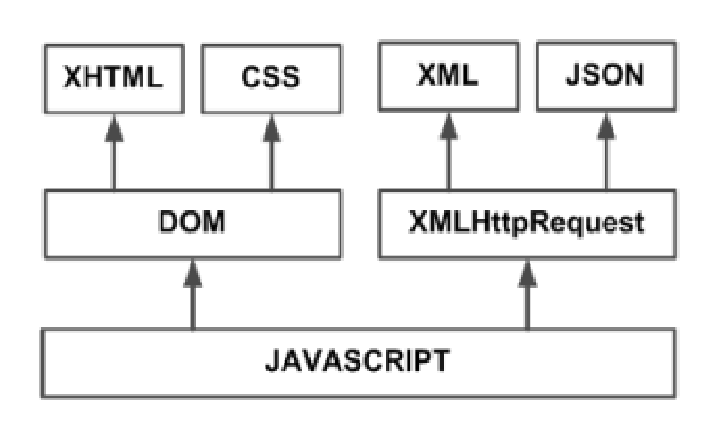
\includegraphics[width=9cm]{./eps/tecnologias/ajax_tecnologias_agrupadas.eps}
        \caption{Tecnologías agrupadas bajo el concepto de AJAX}
        \label{fig:tec_ajax_techs}
      \end{figure}
      
   El modelo clásico de aplicaciones Web funciona de esta forma: La mayoría de las acciones del usuario en la interfaz disparan un requerimiento HTTP al servidor web. El servidor efectúa un proceso (recopila información, procesa números, hablando con varios sistemas propietarios), y le devuelve una pagina HTLM al cliente.
   
   En la figura \ref{fig:tec_ajax_trad_vs_nuevo}, la imagen de la izquierda muestra el modelo tradicional de las aplicaciones web. La imagen de la derecha muestra el nuevo modelo propuesto por AJAX:
   
   \begin{figure}[H]
     \centering
       \includegraphics[width=10cm]{./eps/tecnologias/ajax_comparacion.eps}
     \caption{Comparación gráfica del modelo tradicional de aplicación web y del nuevo modelo propuesto por AJAX}
     \label{fig:tec_ajax_trad_vs_nuevo}
   \end{figure}   
   
   Esta técnica tradicional para crear aplicaciones web funciona correctamente, pero no crea una buena sensación al usuario. Al realizar peticiones continuas al servidor, el usuario debe esperar a que se recargue la página con los cambios solicitados. Si la aplicación debe realizar peticiones continuas, su uso se convierte en algo molesto

   AJAX permite mejorar completamente la interacción del usuario con la aplicación, evitando las recargas constantes de la página, ya que el intercambio de información con el servidor se produce en un segundo plano.

   Las aplicaciones construidas con AJAX eliminan la recarga constante de páginas mediante la creación de un elemento intermedio entre el usuario y el servidor. La nueva capa intermedia de AJAX mejora la respuesta de la aplicación, ya que el usuario nunca se encuentra con una ventana del navegador vacía esperando la respuesta del servidor.

   El siguiente esquema (figura \ref{fig:tec_ajax_comparaciones}) muestra la diferencia más importante entre una aplicación web tradicional y una aplicación web creada con AJAX. La imagen superior muestra la interación síncrona propia de las aplicaciones web tradicionales. La imagen inferior muestra la comunicación asíncrona de las aplicaciones creadas con AJAX.
   
   \begin{figure}[H]
      \centering
        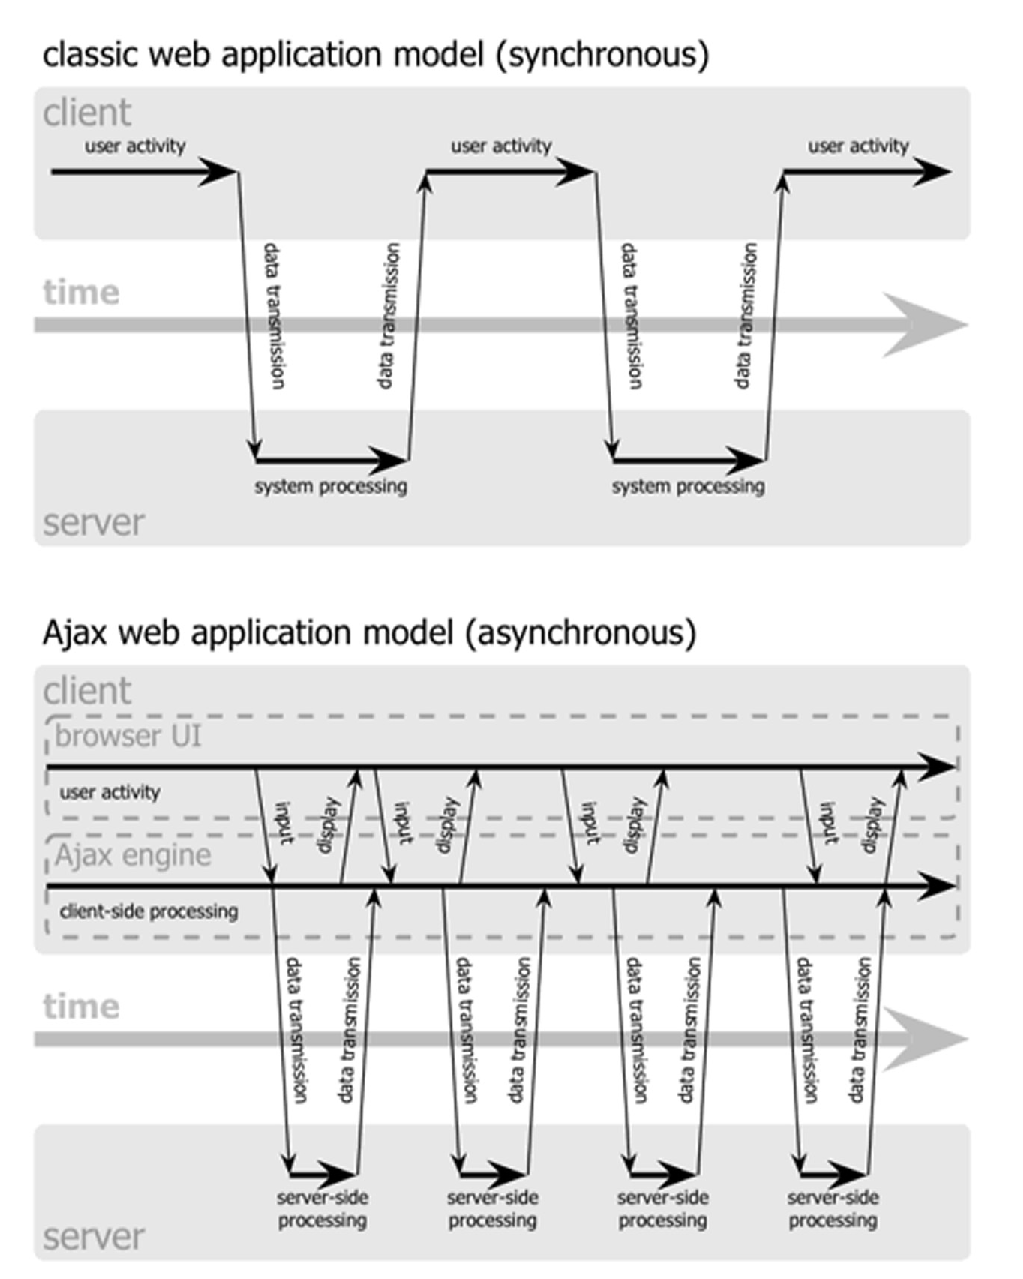
\includegraphics[width=10cm]{./eps/tecnologias/ajax_comunicaciones.eps}
      \caption{Comparación entre las comunicaciones síncronas de las aplicaciones web tradicionales y las comunicaciones asíncronas de las aplicaciones AJAX}
      \label{fig:tec_ajax_comparaciones}
    \end{figure}
    
    Las peticiones HTTP al servidor se sustituyen por peticiones JavaScript que se realizan al elemento encargado de AJAX. Las peticiones más simples no requieren intervención del servidor, por lo que la respuesta es inmediata. Si la interacción requiere una respuesta del servidor, la petición se realiza de forma asíncrona mediante AJAX. En este caso, la interacción del usuario tampoco se ve interrumpida por recargas de página o largas esperas por la respuesta del servidor.

    Desde su aparición, se han creado cientos de aplicaciones web basadas en AJAX. En la mayoría de casos, AJAX puede sustituir completamente a otras técnicas como Flash. Además, en el caso de las aplicaciones web más avanzadas, pueden llegar a sustituir a las aplicaciones de escritorio.
  
  % subsection ajax (end)
  
% section tecnologías (end)


%
% FIN DEL CAPÍTULO
%
\newpage
\thispagestyle{empty}